

%% ----------------------------
%% 1. CONFIGURACIÓN BÁSICA DEL DOCUMENTO
%% ----------------------------
\usepackage{mathtools}                  % Mejoras para matemáticas, incluye amsmath
                                        % va antes de abel, por conflictos inline con \int, \sum, etc.
\ifdefined\HCode
    \usepackage[spanish,english]{babel} % NO CAMBIAR: make4ht necesita english
    \usepackage[T1]{fontenc}            % Para fuentes con acentos correctamente
    \usepackage[utf8]{inputenc}         % Si usas LaTeX clásico
\else
    \usepackage[spanish,english, es-noquoting]{babel}
    \usepackage[autostyle, spanish = mexican]{csquotes} % Manejo de comillas
    \MakeOuterQuote{"}
    \usepackage[T1]{fontenc}
    \usepackage[utf8]{inputenc} % Para fuentes con acentos correctamente
    \decimalpoint % Cambiar a punto
\fi

%% ----------------------------
%%  "GEOMETRÍA" DE LA HOJA
%% ----------------------------
\RequirePackage[a4paper, top=2cm, bottom=2cm, left=2cm, right=2cm, headsep=10pt]{geometry}
%% ----------------------------
%%  PAQUETES BÁSICOS
%% ----------------------------
\RequirePackage{adjustbox}
\RequirePackage{changepage}                 % Ajuste de márgenes
\RequirePackage[table]{xcolor}
% Opciones para los caption
\RequirePackage[labelfont=bf,font=small]{caption}
% Cabeceras bonitas
\RequirePackage{fancyhdr}
% Comandos con opciones
\RequirePackage{xargs}
\RequirePackage{xparse}					% \NewDocumentEnvironment
% Tablas más bonitas
\RequirePackage{booktabs}
%Para opciones de los títulos de sección
\RequirePackage{titlesec}
%% ----------------------------
%%  HIPERVÍNCULOS Y REFERENCIAS
%% ----------------------------
\RequirePackage{hyperref}
%\usepackage{hyperref}                   % Hipervínculos
\definecolor{ligas}{HTML}{0000EE}       % Color para enlaces
\hypersetup{
    colorlinks=true,
    urlcolor=ligas,
    linkcolor=ligas,
    citecolor=ligas,
    hyperindex=true,
    linktoc=all
}
%% ----------------------------
%%  CONFIGURACIÓN DE TEXTO, FUENTES, ENUMERACION, CAPTION
%% ----------------------------
\ifdefined\HCode\else % fuentes PDFLATEX -> pdf
%\RequirePackage{pslatex}                              % Fuentes finas postscript
%\RequirePackage[sc]{mathpazo}                         % Fuentes mathpazo
\RequirePackage{palatino}
\RequirePackage{tgpagella}
%\RequirePackage{eulerpx}
\RequirePackage{eucal}
\RequirePackage[scaled=0.83]{beramono}
%\RequirePackage{chancery}
\RequirePackage{helvet}
\setlength{\parskip}{12pt} % El espacio en el HTML se definió en config.cfg
\fi
\parindent=0mm
\usepackage[fixed]{fontawesome5}        % Iconos modernos
\usepackage{longtable}
\usepackage{latexsym, stmaryrd}         % Símbolos matemáticos adicionales
\usepackage{amssymb, amsthm}   % Paquetes AMS estándar
%\let\openbox\relax % Eliminar el cuadrado al final de una prueba con "proof"
% proof
\renewcommand{\qedsymbol}{\textcolor{razul}{\rule{1.2ex}{1.2ex}}}




%----------------------------


\usepackage[labelfont=bf, font=small]{caption} % Configuración de caption
\usepackage{subcaption}                 % Subfiguras
%Redefinir itemize como enumerate con bullets
\usepackage{enumitem}

% Redefinir itemize para que sea enumerate con números
\let\olditemize\itemize
\let\oldenditemize\enditemize
\renewenvironment{itemize}{%
  \begin{enumerate}%
}{%
  \end{enumerate}%
}
%% ----------------------------
%%  COLORES
%% ----------------------------
\definecolor{nota}{rgb}{0.83, 0.18, 0.18}         % Rojo intenso (\#D32F2F)
\definecolor{fgray}{RGB}{251, 251, 251}
\definecolor{ffgray}{rgb}{.7,.7,.7}
\definecolor{blanco}{RGB}{255,255,255}
\definecolor{c666666}{RGB}{102,102,102}
\definecolor{ca7b1a6}{RGB}{167,177,166}
\definecolor{c100f0d}{RGB}{16,15,13}
% Color para los t\'itulos de las secciones y subsecciones
\definecolor{fazul}{RGB}{245, 245, 240}   % Azul original (0, 0, 153) con 5% de opacidad
\definecolor{razul}{RGB}{0,0,128}
\definecolor{azulEntornos}{rgb}{.0,.0,.3}
\definecolor{azulTitulos}{RGB}{37,74,165}
\definecolor{amarilloEntornos}{RGB}{248,248,245}
\definecolor{amarilloLema}{RGB}{255,202,0}
\definecolor{azulNota}{RGB}{68,0,170}
\definecolor{amarilloCaja}{RGB}{251,237,121}
\definecolor{fntGris}{rgb}{.3,.3,.3}
\definecolor{fntVerde}{RGB}{0,50,0}
\definecolor{tverde}{HTML}{176B3B}
\definecolor{torange}{HTML}{993C00}
\definecolor{headerblue}{RGB}{0, 82, 147}
\definecolor{rowgray}{RGB}{242, 242, 242}
\definecolor{highlight}{RGB}{255, 215, 0}
% Color para entornos (en este documento no se usan todos)
\definecolor{definicion}{rgb}{0.18, 0.49, 0.20}   % Verde oscuro (#2E7D32)
\definecolor{teorema}{rgb}{0.96, 0.49, 0.00}      % Naranja (#F57C00)
\definecolor{ejemplo}{rgb}{0.10, 0.46, 0.82}      % Azul fuerte (#1976D2)
\definecolor{nota}{rgb}{0.83, 0.18, 0.18}         % Rojo intenso (#D32F2F)
\definecolor{lema}{rgb}{1.00, 0.60, 0.00}         % Naranja claro (#FF9800)
\definecolor{corolario}{rgb}{0.98, 0.75, 0.18}    % Amarillo dorado (#FBC02D)
\definecolor{axioma}{rgb}{0.72, 0.11, 0.11}       % Rojo oscuro (#B71C1C)
\definecolor{conjetura}{rgb}{0.48, 0.12, 0.64}    % Morado (#7B1FA2)
\definecolor{problema}{rgb}{0.90, 0.32, 0.00}     % Naranja oscuro (#E65100)
\definecolor{casoespecial}{rgb}{0.40, 0.73, 0.42} % Verde claro (#66BB6A)
\definecolor{advertencia}{rgb}{0.78, 0.15, 0.15}  % Rojo fuerte (#C62828)
\definecolor{aplicacion}{rgb}{0.26, 0.65, 0.96}   % Azul celeste (#42A5F5)
\definecolor{historia}{rgb}{0.48, 0.34, 0.27}     % Marrón (#795548)
\definecolor{explicacionalt}{rgb}{0.00, 0.53, 0.48} % Verde azulado (#00897B)
\definecolor{referenciacruzada}{rgb}{0.26, 0.26, 0.26} % Gris oscuro (#424242)
\definecolor{proyecto}{rgb}{0.05, 0.28, 0.63}     % Azul oscuro (#0D47A1)
\definecolor{cita}{rgb}{0.98, 0.55, 0.00}         % Naranja suave (#FB8C00)
\definecolor{bibliografia}{rgb}{0.38, 0.38, 0.38} % Gris medio (#616161)
\definecolor{nota}{rgb}{0.83, 0.18, 0.18}         % Rojo intenso (\#D32F2F)
\definecolor{actividad}{rgb}{0.55, 0.83, 0.37}         % Rojo intenso (\#D32F2F)
%% ----------------------------
%% 5. ELEMENTOS GRÁFICOS
%% ----------------------------
\usepackage{tikz}                       % Gráficos vectoriales
\usetikzlibrary{matrix}                 % Funcionalidad adicional para TikZ
%\def\pgfsysdriver{pgfsys-dvisvgm4ht.def}% para responsividad html
\usepackage{adjustbox}                  % Ajuste de cajas
\usepackage{changepage}                 % Ajuste de márgenes
\usepackage{array, booktabs}            % Tablas profesionales
\usepackage{multirow}                   % Celdas multi-fila
\newcolumntype{P}[1]{>{\centering\arraybackslash}p{#1}} % Columna centrada
%% ----------------------------
%% PAQUETES ESENCIALES
%% ----------------------------
\usepackage{float}                      % Posicionamiento de figuras/tablas
\usepackage{lipsum}                     % Texto de relleno
\usepackage{multicol}                   % Múltiples columnas
\usepackage{iftex}                      % Detección del motor de compilación
\usepackage[numbers]{natbib}            % Bibliografía [1],[2]                     % Más opciones para comandos
\usepackage{environ}                    % Entornos personalizados
\usepackage{etoolbox}                   % Herramientas para programación
\usepackage{cancel}                     % Para tachar términos matemáticos
\usepackage{bbm}
\ifdefined\HCode % Paquete de ejercicios exsheets, actualmente no soportado por Make4ht, solo PDFLatex
\else %solo PDFLatex
\usepackage[counter-format=se.qu,counter-within=section]{exsheets}
\DeclareTranslation{english}{exsheets-exercise-name}{\textcolor{tverde}{Ejercicio}}
 \DeclareTranslation{english}{exsheets-question-name}{\textcolor{tverde}{Pregunta}}
 \DeclareTranslation{english}{exsheets-solution-name}{\textcolor{tverde}{Solución}}
\SetupExSheets{
	question/pre-body-hook = {\normalfont},
	solution/pre-hook = {\par\medskip},
}
\fi

%% ----------------------------
%% LISTADOS DE CÓDIGO: LISTINGS
%% ----------------------------
\RequirePackage{listings}
\lstset{captionpos=t}
\renewcommand{\lstlistingname}{C\'odigo} % Es importante el acento de esa manera

% Definir colores personalizados para listings
\definecolor{mauve}{rgb}{0.58,0,0.82}
\definecolor{codegreen}{rgb}{0,0.6,0}
\definecolor{codegray}{rgb}{0.5,0.5,0.5}
\definecolor{codepurple}{rgb}{0.58,0,0.82}
\definecolor{backcolour}{rgb}{0.99,0.99,0.99}
\definecolor{lstgray}{RGB}{251, 251, 251}
% Configuración del entorno listings
%\renewcommand{\ttdefault}{pcr}

\captionsetup[lstlisting]{%
  %font=small, % Hace que el texto del caption sea pequeño
  labelfont=bf, % Hace que el "Listado X" sea negrita
  %textfont=bf % Hace que el texto del caption sea negrita
  %justification=raggedright, % <--- Alinea el caption a la izquierda
  %singlelinecheck=false % Importante: asegura que se aplique incluso si es una sola línea
}
\lstset{
    language={[latex]TeX}, % Lenguaje LaTeX
    backgroundcolor=\color{backcolour}, % Color de fondo
    basicstyle=\small\fontseries{b}\ttfamily, % Estilo básico
    breakatwhitespace=false, % No romper líneas en espacios en blanco
    breaklines=true, % Romper líneas largas
    commentstyle=\color{mauve}, % Estilo de los comentarios
    %deletekeywords={...}, % Palabras clave a eliminar
    escapeinside={\%*}{*)}, % Escapar dentro del código
     extendedchars=true, % Caracteres extendidos
     frame=single, % Marco alrededor del código
    keepspaces=true, % Mantener espacios
     moredelim=[is][\color{red}]{\%*}{*\%}, % Delimitador personalizado
 keywordstyle=\color{blue}, % Estilo de las palabras clave
 morekeywords={*,usepackage,begin,end, lstinline, newenvironment,
 	tabular, minipage, pmatrix,bmatrix, includegraphics,captionof,width,scale,rowcolor,multirow,multicolumn, documentclass, input,ifdefined, HCode,Configure,fi, ConfigureEnv,insertarhtml, ifvmode,label,Css,pdfomk,ejersol,hejersol},
    texcsstyle=[1]\color{blue},%label, caption, etc.
     numbers=none,
     %numbers=left, % Números de línea a la izquierda
     %numbersep=5pt, % Separación de los números de línea
     %numberstyle=\tiny\color{codegray}, % Estilo de los números de línea
     rulecolor=\color{gray}, % Color de la regla
     showspaces=false, % No mostrar espacios
     showstringspaces=false, % No mostrar espacios en cadenas
     showtabs=false, % No mostrar tabulaciones
     %stepnumber=1, % Paso de los números de línea
     stringstyle=\color{mauve}, % Estilo de las cadenas
     % NO Habilitar title=\lstname
     literate= {∩}{{$\cap$}}1 {á}{{\'a}}1 {é}{{\'e}}1 {í}{{{\'\i}}}1 {ó}{{\'o}}1 {ö}{{\"o}}1 {ő}{{\H o}}1 {ú}{{\'u}}1 {Ú}{{\'U}}1 {ü}{{\"u}}1 {ű}{{\H u}}1 {Ü}{{\"U}}1
}
%%--listing

%% ----------------------------
%% FUENTES PERSONALIZADAS
%% ----------------------------
\newcommand{\htmlusefont}[1]{% Make4ht -> html
  \HCode{<span class="ptsansnarrow">}#1\HCode{</span>}%
}
\newcommand{\fhvb}[2]{{\fontfamily{phv}\fontseries{b}\fontsize{#1}{1}\selectfont{#2}}}
\newcommand{\fhv}[2]{{\fontfamily{phv}\fontsize{#1}{1}\selectfont{#2}}}
\newcommand{\fvnp}[1]{\fhvb{10}{#1}}
\newcommand{\fte}[1]{\fhvb{10}{\textcolor{razul}{#1}}}
\newcommand{\fvn}[1]{\fhv{10}{#1}}
\newcommand{\fvns}[1]{\fhv{10}{#1}}
\newcommand{\fvntt}[1]{\fhv{10}{#1}}
\newcommandx{\fntg}[4][1=pag,2=9,3=n]{{\color{fntGris}\fontfamily{#1}\fontsize{#2}{1}\fontshape{#3}\selectfont{#4}}}
\newcommandx{\fnte}[4][1=phv,2=9,3=n]{{\color{fntVerde}\fontfamily{#1}\fontsize{#2}{1}\fontshape{#3}\selectfont{#4}}}
\newcommand{\ofvnp}[1]{\textcolor{torange}{\fvnp{#1}}}
\renewcommand{\tt}[1]{\textcolor{tverde}{\fvntt{#1}}}
\newcommand{\wtt}[1]{\textcolor{torange}{\fvntt{#1}}}
%--------------------------


%%-- TITULO - FECHA - AUTORES - RESUMEN - ABSTRACT - KEYWORDS - etc.
%--------------------------------------------------------------------------
%.: Título PDFLatex :.
\newcommand{\titulo}[6]{%espanol-ingl\'es-volumen-n\'umero-mes de inicio[, anno]-mes final, anno
	\title{
		\thispagestyle{empty}
		\headerInicial{Vol\; #3, \;No #4.   #5\,-\,#6}
		\begin{center}
			{\Large\bfseries #1}\\[0.22cm]
			{\usefont{T1}{PTSansNarrow-TLF}{}{n} | {\normalsize #2} |}
		\end{center}
		% Habilita las cabeceras en las páginas (con ese dise\~no)
		\revistaheaderA{Vol\; #3,\;No \;#4.  #5\,-\,#6}
		\medskip
	}
}
\newcommand{\headerInicial}[1]{
	\vspace{-2cm}
	\textcolor{lightgray}{\rule[0.5cm]{\textwidth}{4pt}}\\[-0.2cm]
	\begin{minipage}{0.1\textwidth}
		
\includegraphics[width=1.4cm]{images/logo}
	\end{minipage}
	\begin{minipage}{0.85\textwidth}
		\fhv{10}{Revista digital }\\[-0.3cm]
		\fhvb{10}{Matem\'atica, Educaci\'on e Internet\hfill \fntg[phv][8]{
\includegraphics[scale=0.8]{images/logocc.png}}\\[-0.3cm]
			\fvn{%
				\href{https://revistas.tec.ac.cr/index.php/matematica}{https://revistas.tec.ac.cr/index.php/matematica}}\hfill \fntg[phv][8]{ISSN 1659 -0643}}\\[-0.3cm]
		\fvn{#1} \hfill \fntg[phv][8]{DOI: \href{https://doi.org/10.18845/rdmei.v26i2.8214}{10.18845/rdmei.v26i2.8214}}
	\end{minipage}
	\textcolor{lightgray}{\rule[0.5cm]{\textwidth}{0.1pt}}
}
%\revistaheaderA{V\lowercase{ol 12, }N\lowercase{o 2. }  M\lowercase{arzo} $-$ A\lowercase{gosto} 2012.}
 \newcommand{\revistaheaderA}[1]{\markboth{R\lowercase{evista digital} M\lowercase{atem\'atica,} E\lowercase{ducaci\'on e} I\lowercase{nternet} \lowercase{\href{https://revistas.tec.ac.cr/index.php/matematica}{\lowercase{(https://revistas.tec.ac.cr/index.php/matematica)}}}. #1}{R\lowercase{evista digital} M\lowercase{atem\'atica,} E\lowercase{ducaci\'on e}I\lowercase{nternet} \lowercase{\href{https://revistas.tec.ac.cr/index.php/matematica}{\lowercase{(https://revistas.tec.ac.cr/index.php/matematica)}}}. #1}}


%--------------------------------------------------------------------------
%% .: TITULO para Make4ht :.
%-------------------------------------------------------------------------
\newcommand{\webtitulo}[6]{%espanol-ingl\'es-volumen-n\'umero-mes de inicio[, anno]-mes final, anno
{ %\begingroup necesario
\setlength{\arrayrulewidth}{6pt}
\arrayrulecolor{lightgray}
%\begin{tabular*}{\textwidth}{@{\extracolsep{\fill}}llr@{}}
\begin{tabular}{@{\extracolsep{\fill}}llr@{}}
\toprule[4pt]
        % --- Primera fila (autores 1, 2, 3) ---
        \begin{efntabular}
        \begin{tabular}[t]{@{}r@{}}
\raisebox{\dimexpr-\height + 1.5ex\relax}{  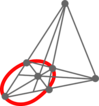
\includegraphics{images/weblogo.png}}
        \end{tabular}%
        \end{efntabular}
            &
            \begin{efntabular}
            \begin{tabular}[t]{@{}l@{}}
    \fhv{10}{Revista digital }\\
    \fhvb{10}{Matem\'atica, Educaci\'on e Internet}\\
    \fntg[phv][9]{\href{https://revistas.tec.ac.cr/index.php/matematica}{https://revistas.tec.ac.cr/index.php/matematica}}\\
    \fhv{10}{Vol\; #3,\;No \;#4.  #5 \,\textminus\,   #6}%\\
            \end{tabular}%
            \end{efntabular}
                &
                \begin{efntabular}
                \begin{tabular}[t]{@{}r@{}}
             \raisebox{\dimexpr-\height + 1.5ex\relax}{ 
\includegraphics{images/weblogocc.png}}\\
    \fntg[phv][8]{ISSN 1659 -0643}\\
   \fntg[phv][8]{DOI: \href{https://doi.org/10.18845/rdmei.v26i2.8214}{10.18845/rdmei.v26i2.8214}}\\
                \end{tabular}%
                \end{efntabular}\\
                \bottomrule
\end{tabular}
}
		\begin{center}
			{\Large\bfseries #1}\\
			\htmlusefont{| #2 |}
		\end{center}
    } % webtitulo

%--------------------------------------------------------------------------
%%-- Recibido - Aceptado
%-------------------------------------------------------------------------
\newcommand{\fecha}[2]{% PDFLaTeX -> pdf
	\date{
		{\textcolor{lightgray}{\rule[0.5cm]{0.8\textwidth}{0.1pt}}} \\[-0.2cm]
		\begin{minipage}{0.6\textwidth}
			\fhv{9}{\color{azulEntornos} Recibido: #1}\hfill\fhv{9}{\color{azulEntornos} Aceptado: #2}  \\[0.04cm]
			{\textcolor{lightgray}{\rule[0.5cm]{\textwidth}{0.1pt}}}
		\end{minipage}
		\vspace{-5mm}
	}
}
\newcommand{\webfecha}[2]{%
  \ifvmode\IgnorePar\fi\EndP
  { % grupo local
   \arrayrulecolor{lightgray}%
   \setlength{\arrayrulewidth}{0.3pt}%
   \begin{tabular*}{\textwidth}{@{\extracolsep{\fill}} p{0.3\textwidth} p{0.4\textwidth} p{0.3\textwidth} }
   \hline
      \HCode{<span style="color:\#1b3a75;">}\fvns{Recibido: #1}\HCode{</span>}
      &\HCode{<span style="display:inline-block; width: 4em;"></span>} & %espacio en la columna 2
      \HCode{<span style="color:\#1b3a75;">}\fvns{Aceptado: #2}\HCode{</span>} \\
    \cline{1-1} \cline{3-3}
  \end{tabular*}
  }
}


% Comando \cejilla
% ═══════════════════════════════════════════════════════════
% CEJILLA - Comando LaTeX para pestañas colapsables
% Uso: \cejilla{nombre}{contenido latex}
% ═══════════════════════════════════════════════════════════

% \newcommand{\webtableofcontents}{%
% \ifvmode\IgnorePar\fi\EndP
% \ifdefined\HCode
% \ifvmode\IgnorePar\fi\EndP
% \ifvmode\IgnorePar\fi\EndP
% \fi
% \ifdefined\HCode
% \ifvmode\IgnorePar\fi\EndP
% \tableofcontents
% \ifvmode\IgnorePar\fi\EndP
% \fi
% \ifdefined\HCode
% \ifvmode\IgnorePar\fi\EndP
% \HCode{</div>}
% \ifvmode\IgnorePar\fi\EndP
% \fi
% }

%% ----------------------------
%% COMANDOS ESPECIALES MAK4HT -> HTML
%% ----------------------------

%1.) Tablas hover...PDFLatex ignora,
%    Make4ht lo aplica:Una envoltura <div class="tabla-hover-filas">...
\newenvironment{tablahoverfilas}
  {%
    \ifdefined\HCode
      \ifvmode\IgnorePar\fi\EndP
      \HCode{<div class="tabla-hover-filas">}%
      \par
    \fi
  }
  {%
    \ifdefined\HCode
      \ifvmode\IgnorePar\fi\EndP
      \HCode{</div>}%
      \par
    \fi
  }
%
% \rowcolor{rowgray} tapa el hover, \rowgris para css y da \rowcolor{rowgray} para pdf
\ifdefined\HCode
  \newcommand{\rowgris}{\HCode{<tr class="rowgray">}}
\else
  \newcommand{\rowgris}{\rowcolor{rowgray}}
\fi
%%--
%2.) \vspace \bigskip, \medskip, \smallskip para html

\newcommand{\linea}{\textcolor{lightgray}{\rule{\linewidth}{0.4pt}}\par}
\ifdefined\HCode
  \def\bigskip{\HCode{<div style="margin-top:2em;"></div>}}
  \def\medskip{\HCode{<div style="margin-top:1.5em;"></div>}}
  \def\smallskip{\HCode{<div style="margin-top:1em;"></div>}}
  \def\linea{\HCode{<hr style="height:1px; border:none; background-color:\#ccc; margin:20px 0;">}}
\fi
%
\ifdefined\HCode
  \newcommand{\vspacehtml}[1]{\HCode{<div style="margin-top:#1;"></div>}}
\else
  \newcommand{\vspacehtml}[1]{\vspace*{#1}}
\fi
%% \vspacehtml{1em}
%%--
% 3.) Comandos \pdfomk{#1}{#2} e \insertarhtml{}

\ifdefined\HCode
  \long\def\solopdf#1{\protect}  % ignorado por make4ht
  \long\def\solomk#1{\protect#1} % procesado en make4ht
\else
  \long\def\solopdf#1{\protect#1} % procesado en PDF
  \long\def\solomk#1{\protect}    % ignorado por PDF
\fi

% 3a.) \pdfomk{#1}{#2}
\ifdefined\HCode
\long\def\pdfomk#1#2{%
	\protect#2%html
}
\else
\long\def\pdfomk#1#2{%
	\protect#1%pdf
}
\fi
%-3b.)--Insertar html
%
%--\insertarhtml{#1} %Para html PURO
  \ifdefined\HCode
    \long\def\insertarhtml#1{%
      \HCode{#1}%
    }
  \else
    \long\def\insertarhtml#1{%
      %nada%\textbf{[Contenido interactivo no disponible en PDF]}
    }
  \fi
%
%- 4.) Un entorno para ejercicio con botón para ver/ocultar respuesta
%
\newcounter{htmlEjercicio}[section]
\renewcommand{\thehtmlEjercicio}{%
  \ifnum\value{section}=0
    \arabic{htmlEjercicio}%
  \else
    \thesection.\arabic{htmlEjercicio}%
  \fi
}
% Nota: Debemos poner \insertarhtml{<script src="js/ejerciciosolucion.js" defer></script>}
% antes de \end{document}
% para que el script quede al  final del documento (justo antes de cerrar </body>),
% así todos los elementos HTML ya han sido parseados y existen en el DOM.
% Por lo tanto, document.querySelectorAll(".ejercicio-solucion button") puede encontrar
% los botones correctamente.
% \insertarhtml{<script src="js/ejerciciosolucion.js" defer></script>}
\ifdefined\HCode
\newcommand{\hejersol}[2]{%
    \stepcounter{htmlEjercicio}%
    \par\medskip
        \ifvmode\IgnorePar\fi\EndP
    \noindent\textbf{Ejercicio \thehtmlEjercicio}
    #1%
        \ifvmode\IgnorePar\fi\EndP
    \HCode{%
      <div class="ejercicio-solucion">
        <div class="solucion-container">
          <button onclick="this.nextElementSibling.classList.toggle('visible')">Mostrar/Ocultar solución</button>
          <div class="solucion">
          %<script src="js/ejerciciosolucion.js"></script>
    }%
        \ifvmode\IgnorePar\fi\EndP
    #2%
        \ifvmode\IgnorePar\fi\EndP
    \HCode{</div></div></div>}%
    \par\medskip
  }
\else
  \newcommand{\hejersol}[2]{%
    % No imprimir nada en PDF
  }
\fi
%%-- pdf-exsheet y make4ht
% Definición base para PDF (LaTeX estándar)
\newcommand{\ejersol}[2]{%[4][]{%  % #1 = opciones para question (opcional)
    \begin{question}%[#1]%
        #1%                    % #3 = enunciado
    \end{question}%
    \begin{solution}%[print=true]%  % Opción FIJADA para evitar errores
        #2%                    % #4 = solución
    \end{solution}%
}

% Sobrescribir para make4ht (HTML)
\ifdefined\HCode
    \renewcommand{\ejersol}[2]{\hejersol{#1}{#2}}  % Ignora opciones en HTML
\fi


%%------------------------------
% .: TABLA AUTORES PDFLATEX - MAKE4HT
%%-------------------------------

\newcommand{\autor}[5]{% Nombre - email - Universidad - Pa\'is - N\'umero de ORCID
	\def\nombreautoruno{#1}
	\def\correoautoruno{#2}
	\def\universidadautoruno{#3}
	\def\paisautoruno{#4}
	\def\orcidautoruno{#5}
}

\newcommand{\autordos}[5]{% Nombre - email - Universidad - Pa\'is - N\'umero de ORCID
	\def\nombreautordos{#1}
	\def\correoautordos{#2}
	\def\universidadautordos{#3}
	\def\paisautordos{#4}
	\def\orcidautordos{#5}
}

\newcommand{\autortres}[5]{% Nombre - email - Universidad - Pa\'is - N\'umero de ORCID
	\def\nombreautortres{#1}
	\def\correoautortres{#2}
	\def\universidadautortres{#3}
	\def\paisautortres{#4}
	\def\orcidautortres{#5}
}

\newcommand{\autorcuatro}[5]{% Nombre - email - Universidad - Pa\'is - N\'umero de ORCID
	\def\nombreautorcuatro{#1}
	\def\correoautorcuatro{#2}
	\def\universidadautorcuatro{#3}
	\def\paisautorcuatro{#4}
	\def\orcidautorcuatro{#5}
}

\newcommand{\autorcinco}[5]{% Nombre - email - Universidad - Pa\'is - N\'umero de ORCID
	\def\nombreautorcinco{#1}
	\def\correoautorcinco{#2}
	\def\universidadautorcinco{#3}
	\def\paisautorcinco{#4}
	\def\orcidautorcinco{#5}
}

\newcommand{\autorseis}[5]{% Nombre - email - Universidad - Pa\'is - N\'umero de ORCID
	\def\nombreautorseis{#1}
	\def\correoautorseis{#2}
	\def\universidadautorseis{#3}
	\def\paisautorseis{#4}
	\def\orcidautorseis{#5}
}

\newcommand{\autorsiete}[5]{% Nombre - email - Universidad - Pa\'is - N\'umero de ORCID
	\def\nombreautorsiete{#1}
	\def\correoautorsiete{#2}
	\def\universidadautorsiete{#3}
	\def\paisautorsiete{#4}
	\def\orcidautorsiete{#5}
}

\newcommand{\autorocho}[5]{% Nombre - email - Universidad - Pa\'is - N\'umero de ORCID
	\def\nombreautorocho{#1}
	\def\correoautorocho{#2}
	\def\universidadautorocho{#3}
	\def\paisautorocho{#4}
	\def\orcidautorocho{#5}
}

\newcommand{\autores}{% Nombre - email - Universidad - Pa\'is - N\'umero de ORCID
	\author{
		\fnte[phv][12]{\href{https://orcid.org/\orcidautoruno}{
\includegraphics[scale=0.65]{./images/ORCID-iD_icon-16x16.png}} \nombreautoruno}\\
		\fvn{\correoautoruno}\\
		\fvn{\universidadautoruno} \\
		\fvn{\paisautoruno} \\
		\ifx\nombreautordos\undefined\else
			\and
			\fnte[phv][12]{\href{https://orcid.org/\orcidautordos}{
\includegraphics[scale=0.65]{./images/ORCID-iD_icon-16x16.png}} \nombreautordos}\\
			\fvn{\correoautordos}\\
			\fvn{\universidadautordos} \\
			\fvn{\paisautordos} \\
			\ifx\nombreautortres\undefined\else
				\and
				\fnte[phv][12]{\href{https://orcid.org/\orcidautortres}{
\includegraphics[scale=0.65]{./images/ORCID-iD_icon-16x16.png}} \nombreautortres}\\
				\fvn{\correoautortres}\\
				\fvn{\universidadautortres} \\
				\fvn{\paisautortres} \\
				\ifx\nombreautorcuatro\undefined\else
					\and
					\fnte[phv][12]{\href{https://orcid.org/\orcidautorcuatro}{
\includegraphics[scale=0.65]{./images/ORCID-iD_icon-16x16.png}} \nombreautorcuatro}\\
					\fvn{\correoautorcuatro}\\
					\fvn{\universidadautorcuatro} \\
					\fvn{\paisautorcuatro} \\
					\ifx\nombreautorcinco\undefined\else
						\and
						\fnte[phv][12]{\href{https://orcid.org/\orcidautorcinco}{
\includegraphics[scale=0.65]{./images/ORCID-iD_icon-16x16.png}} \nombreautorcinco}\\
						\fvn{\correoautorcinco}\\
						\fvn{\universidadautorcinco} \\
						\fvn{\paisautorcinco} \\
						\ifx\nombreautorseis\undefined\else
							\and
							\fnte[phv][12]{\href{https://orcid.org/\orcidautorseis}{
\includegraphics[scale=0.65]{./images/ORCID-iD_icon-16x16.png}} \nombreautorseis}\\
							\fvn{\correoautorseis}\\
							\fvn{\universidadautorseis} \\
							\fvn{\paisautorseis} \\
							\ifx\nombreautorsiete\undefined\else
								\and
								\fnte[phv][12]{\href{https://orcid.org/\orcidautorsiete}{
\includegraphics[scale=0.65]{./images/ORCID-iD_icon-16x16.png}} \nombreautorsiete}\\
								\fvn{\correoautorsiete}\\
								\fvn{\universidadautorsiete} \\
								\fvn{\paisautorsiete} \\
								\ifx\nombreautorocho\undefined\else
									\and
									\fnte[phv][12]{\href{https://orcid.org/\orcidautorocho}{
\includegraphics[scale=0.65]{./images/ORCID-iD_icon-16x16.png}} \nombreautorocho}\\
									\fvn{\correoautorocho}\\
									\fvn{\universidadautorocho} \\
									\fvn{\paisautorocho} \\
								\fi
							\fi
						\fi
					\fi
				\fi
			\fi
		\fi
	}
}

%% web autores----------------------------------
\newcommand{\webautores}{%
  \HCode{<div class="autores-container">}%
  \ifdefined\nombreautoruno
    \HCode{<div class="autor">}
    \fnte[phv][12]{\href{https://orcid.org/\orcidautoruno}{
\includegraphics[scale=0.65]{./images/ORCID-iD_icon-16x16.png}} \nombreautoruno}\\
    \fvns{\correoautoruno}\\
    \fvns{\universidadautoruno}\\
    \fvns{\paisautoruno}
    \HCode{</div>}%
  \fi
  \ifdefined\nombreautordos
    \HCode{<div class="autor">}
    \fnte[phv][12]{\href{https://orcid.org/\orcidautordos}{
\includegraphics[scale=0.65]{./images/ORCID-iD_icon-16x16.png}} \nombreautordos}\\
    \fvns{\correoautordos}\\
    \fvns{\universidadautordos}\\
    \fvns{\paisautordos}
    \HCode{</div>}%
  \fi
  \ifdefined\nombreautortres
    \HCode{<div class="autor">}
    \fnte[phv][12]{\href{https://orcid.org/\orcidautortres}{
\includegraphics[scale=0.65]{./images/ORCID-iD_icon-16x16.png}} \nombreautortres}\\
    \fvns{\correoautortres}\\
    \fvns{\universidadautortres}\\
    \fvns{\paisautortres}
    \HCode{</div>}%
  \fi
  \ifdefined\nombreautorcuatro
    \HCode{<div class="autor">}
    \fnte[phv][12]{\href{https://orcid.org/\orcidautorcuatro}{
\includegraphics[scale=0.65]{./images/ORCID-iD_icon-16x16.png}} \nombreautorcuatro}\\
    \fvns{\correoautorcuatro}\\
    \fvns{\universidadautorcuatro}\\
    \fvns{\paisautorcuatro}
    \HCode{</div>}%
  \fi
  \ifdefined\nombreautorcinco
    \HCode{<div class="autor">}
    \fnte[phv][12]{\href{https://orcid.org/\orcidautorcinco}{
\includegraphics[scale=0.65]{./images/ORCID-iD_icon-16x16.png}} \nombreautorcinco}\\
    \fvns{\correoautorcinco}\\
    \fvns{\universidadautorcinco}\\
    \fvns{\paisautorcinco}
    \HCode{</div>}%
  \fi
  \HCode{</div>}%
}

%% ----------------------------
%%  ENTORNOS DE RESUMEN Y ABSTRACT
%% ----------------------------

\renewenvironment{abstract}
{\par\noindent\textcolor{azulTitulos}{\fvnp{Abstract:}}\ \ignorespaces}
{\par\noindent\ignorespacesafterend}


\newenvironment{resumen}{%
{\par\noindent\textcolor{azulTitulos}{\fvnp{Resumen:}}\ \ignorespaces}}


\newenvironment{palabrasclave}{%
{\par\noindent\textcolor{azulTitulos}{\fvnp{Palabras Clave:}}\ \ignorespaces}}


\newenvironment{keywords}{%
{\par\noindent\textcolor{azulTitulos}{\fvnp{Keywords:}}\ \ignorespaces}}

%% ----------------------------
%% ENTORNOS PERSONALIZADOS
%% ----------------------------
\usepackage[framemethod=default]{mdframed} % Cajas con estilo

%% Configuración de estilos para entornos
\mdfdefinestyle{mdframed-fondoblanco}{
    backgroundcolor=blanco,
    linewidth=0pt,
    leftmargin=0pt,
    rightmargin=0pt,
    innerleftmargin=4pt,
    innerrightmargin=4pt,
    innertopmargin=6pt,
    innerbottommargin=0pt,
    skipabove=10pt,
    skipbelow=10pt,
    topline=false,
    bottomline=false,
    rightline=false,
    leftline=false,
    linecolor=blanco
}



%%-- ENTORNOSCON ARGUMENTO OPCIONAL Y SIN LLAVES
% \label{ent:ent1}
%\begin{entorno}[opcional]
%	...contenido
%\end{entorno}

%.: DEFINICION :.
\newcounter{definicion}
\mdfdefinestyle{mdframed-definicion}{%
	 backgroundcolor=blanco,%
	linewidth=0pt,%
	leftmargin=0pt,%
	rightmargin=0pt,%
	innerleftmargin=4pt,%
	innerrightmargin=4pt,%
	innertopmargin=6pt,%
	innerbottommargin=6pt,%
	skipabove=10pt,%
	skipbelow=10pt,%
	linecolor=razul,%
	topline=false,%
	bottomline=false,%
	rightline=false,%
	leftline=true,%
	linewidth=4pt%
}%
%
\NewDocumentEnvironment{definicion}{o}{%
	\refstepcounter{definicion}%
	\begin{mdframed}[style=mdframed-definicion]%
		\textcolor{razul}{\sffamily\textbf{Definición~\thedefinicion\IfValueT{#1}{~(#1)}.}}%
		\par\noindent\ignorespaces
	}{%
	\end{mdframed}%
}

%.: TEOREMA :.
%
\mdfdefinestyle{mdframed-teorema}{
	 backgroundcolor=lightgray!10!white,
	linewidth=0pt,
	leftmargin=0pt,
	rightmargin=0pt,
	innerleftmargin=4pt,
	innerrightmargin=4pt,
	innertopmargin=6pt,
	innerbottommargin=6pt,
	skipabove=10pt,
	skipbelow=10pt,
	linecolor=razul,
	topline=true,
	bottomline=false,
	rightline=false,
	leftline=false,
	linewidth=4pt
}
%
\newcounter{teorema}
\NewDocumentEnvironment{teorema}{o}{%
	\refstepcounter{teorema}%
	\begin{mdframed}[style=mdframed-teorema]%
		\textcolor{razul}{\sffamily\textbf{Teorema~\theteorema\IfValueT{#1}{~(#1)}.}}%
		\vskip0.5pt\relax%
		\noindent\ignorespaces
	}{%
	\end{mdframed}%
% 	 \vskip1pt%
%     {\color{razul}\rule{\linewidth}{1pt}}%  % línea inferior delgada
}
%.: EJEMPLO :.
\mdfdefinestyle{mdframed-ejemplo}{
	 backgroundcolor=blanco,
	linewidth=0pt,
	leftmargin=0pt,
	rightmargin=0pt,
	innerleftmargin=4pt,
	innerrightmargin=4pt,
	innertopmargin=6pt,
	innerbottommargin=6pt,
	skipabove=10pt,
	skipbelow=10pt,
	linecolor=razul,
	topline=false,
	bottomline=false,
	rightline=false,
	leftline=true,
	linewidth=1pt
}
\newcounter{ejemplo}
\NewDocumentEnvironment{ejemplo}{o}{%
	\refstepcounter{ejemplo}%
	\begin{mdframed}[style=mdframed-ejemplo]%
		\textcolor{razul}{\sffamily\textbf{Ejemplo~\theejemplo\IfValueT{#1}{~(#1)}.}}%
		\par\noindent\ignorespaces
	}{%
	\end{mdframed}%
}

%.: CAJA GENERAL :.
\NewDocumentEnvironment{caja}{o}{%
    \begin{mdframed}[
        backgroundcolor=white,
        leftmargin=8pt,
        rightmargin=0pt,
        innerleftmargin=8pt,
        innerrightmargin=0pt,
        innertopmargin=4pt,
        innerbottommargin=4pt,
        skipabove=5pt,
        skipbelow=5pt,
        linecolor=lightgray,
        topline=false,
        bottomline=false,
        rightline=false,
        leftline=false,
        linewidth=0.5pt
    ]
    \textcolor{razul}{%
        \sffamily%
        \textbf{ %blanco
        \IfValueT{#1}{#1.}}% Argumento opcional
    }%
    \ignorespaces \;% Ignora espacios en blanco al inicio
}{
    \end{mdframed}%
}

%.: LEMA :.
\newcounter{lemap}
%\newcounter{steorema}  %usa contador teoremp
\NewDocumentEnvironment{lema}{o}{%
    \refstepcounter{lemap}  %continúa contador teoremp
    \begin{mdframed}[
        backgroundcolor=white,
        linewidth=2pt,
        leftmargin=0pt,
        rightmargin=0pt,
        innerleftmargin=4pt,
        innerrightmargin=4pt,
        innertopmargin=6pt,
        innerbottommargin=0pt,
        skipabove=10pt,
        skipbelow=10pt,
        topline=true,
        bottomline=false,
        rightline=false,
        leftline=false,
        linecolor=lema,
    ]
    \textcolor{black!70!white}{%
        \sffamily%
        \textbf{Lema~\thelemap %
        \IfValueT{#1}{\;(#1)}.}% Argumento opcional
    }
    \ignorespaces
}{%
    \end{mdframed}%
}

%.: COROLARIO :.
\newcounter{corolario}
\NewDocumentEnvironment{corolario}{o}{%
    \refstepcounter{corolario}%
    \begin{mdframed}[
         backgroundcolor=blanco,
        linewidth=0pt,
        leftmargin=0pt,
        rightmargin=0pt,
        innerleftmargin=4pt,
        innerrightmargin=4pt,
        innertopmargin=6pt,
        innerbottommargin=6pt,
        skipabove=10pt,
        skipbelow=10pt,
        linecolor=corolario,
        topline=false,
        bottomline=false,
        rightline=false,
        leftline=true,
        linewidth=2pt
    ]
    \textcolor{black!70!white}{%
        \sffamily%
        \textbf{Corolario~\thecorolario%
        \IfValueT{#1}{~(#1)}.}% Argumento opcional
    }%
    \ignorespaces \;% Ignora espacios en blanco al inicio
}{%
    \end{mdframed}%
}


%.: AXIOMA :.
\NewDocumentEnvironment{axiomas}{o}{%
    \begin{mdframed}[
        backgroundcolor=white,
        leftmargin=0pt,
        rightmargin=0pt,
        innerleftmargin=4pt,
        innerrightmargin=4pt,
        innertopmargin=6pt,
        innerbottommargin=6pt,
        skipabove=10pt,
        skipbelow=10pt,
        linecolor=axioma,
        topline=false,
        bottomline=false,
        rightline=false,
        leftline=true,
        linewidth=2pt
    ]
    \textcolor{axioma!90!black}{%
        \sffamily%
        \textbf{ %blanco
        \IfValueT{#1}{#1.}}% Argumento opcional
    }%
    \ignorespaces \;% Ignora espacios en blanco al inicio
}{%
    \end{mdframed}%
}

%% .: CONJETURA :.
\NewDocumentEnvironment{conjetura}{o}{%
    \begin{mdframed}[
        backgroundcolor=white,
        leftmargin=0pt,
        rightmargin=0pt,
        innerleftmargin=4pt,
        innerrightmargin=4pt,
        innertopmargin=6pt,
        innerbottommargin=6pt,
        skipabove=10pt,
        skipbelow=10pt,
        linecolor=conjetura,
        topline=false,
        bottomline=false,
        rightline=false,
        leftline=true,
        linewidth=2pt
    ]
    \textcolor{conjetura!90!black}{%
        \sffamily%
        \textbf{ %blanco
        \IfValueT{#1}{#1.}}% Argumento opcional
    }%
    \ignorespaces \;% Ignora espacios en blanco al inicio
}{%
    \end{mdframed}%
}

%%-- Entorno problema ejercicio
\NewDocumentEnvironment{problema}{o}{%
    \begin{mdframed}[
        backgroundcolor=problema!5!white,
        leftmargin=0pt,
        rightmargin=0pt,
        innerleftmargin=4pt,
        innerrightmargin=4pt,
        innertopmargin=6pt,
        innerbottommargin=6pt,
        skipabove=10pt,
        skipbelow=10pt,
        linecolor=problema,
        topline=false,
        bottomline=false,
        rightline=false,
        leftline=true,
        linewidth=2pt
    ]
    \textcolor{problema!90!black}{%
        \sffamily%
        \textbf{ %blanco
        \IfValueT{#1}{#1.}}% Argumento opcional
    }%
    \ignorespaces \;% Ignora espacios en blanco al inicio
}{%
    \end{mdframed}%
}
%% .: CASO ESPECIAL :.
\NewDocumentEnvironment{casoespecial}{o}{%
    \begin{mdframed}[
        backgroundcolor=white,
        leftmargin=0pt,
        rightmargin=0pt,
        innerleftmargin=4pt,
        innerrightmargin=4pt,
        innertopmargin=6pt,
        innerbottommargin=6pt,
        skipabove=10pt,
        skipbelow=10pt,
        linecolor=casoespecial,
        topline=false,
        bottomline=false,
        rightline=false,
        leftline=true,
        linewidth=2pt
    ]
    \textcolor{casoespecial!90!black}{%
        \sffamily%
        \textbf{ %blanco
        \IfValueT{#1}{#1.}}% Argumento opcional
    }%
    \ignorespaces \;% Ignora espacios en blanco al inicio
}{%
    \end{mdframed}%
}


%% .: APLICACION :.
\NewDocumentEnvironment{aplicacion}{o}{%
    \begin{mdframed}[
        backgroundcolor=white,
        leftmargin=0pt,
        rightmargin=0pt,
        innerleftmargin=4pt,
        innerrightmargin=4pt,
        innertopmargin=6pt,
        innerbottommargin=6pt,
        skipabove=10pt,
        skipbelow=10pt,
        linecolor=aplicacion,
        topline=false,
        bottomline=false,
        rightline=false,
        leftline=true,
        linewidth=2pt
    ]
    \textcolor{aplicacion!90!black}{%
        \sffamily%
        \textbf{ %blanco
        \IfValueT{#1}{#1.}}% Argumento opcional
    }%
    \ignorespaces \;% Ignora espacios en blanco al inicio
}{%
    \end{mdframed}%
}

%% .: HISTORIA :.
\NewDocumentEnvironment{historia}{o}{%
    \begin{mdframed}[
        backgroundcolor=white,
        leftmargin=0pt,
        rightmargin=0pt,
        innerleftmargin=4pt,
        innerrightmargin=4pt,
        innertopmargin=6pt,
        innerbottommargin=6pt,
        skipabove=10pt,
        skipbelow=10pt,
        linecolor=historia,
        topline=false,
        bottomline=false,
        rightline=false,
        leftline=true,
        linewidth=2pt
    ]
    \textcolor{historia!90!black}{%
        \sffamily%
        \textbf{ %blanco
        \IfValueT{#1}{#1.}}% Argumento opcional
    }%
    \ignorespaces \;% Ignora espacios en blanco al inicio
}{%
    \end{mdframed}%
}


%% .: PROYECTO :.
\NewDocumentEnvironment{proyecto}{o}{%
    \begin{mdframed}[
        backgroundcolor=white,
        leftmargin=0pt,
        rightmargin=0pt,
        innerleftmargin=4pt,
        innerrightmargin=4pt,
        innertopmargin=6pt,
        innerbottommargin=6pt,
        skipabove=10pt,
        skipbelow=10pt,
        linecolor=proyecto,
        topline=false,
        bottomline=false,
        rightline=false,
        leftline=true,
        linewidth=2pt
    ]
    \textcolor{proyecto!90!black}{%
        \sffamily%
        \textbf{ %blanco
        \IfValueT{#1}{#1.}}% Argumento opcional
    }%
    \ignorespaces \;% Ignora espacios en blanco al inicio
}{%
    \end{mdframed}%
}


%% .: ACTIVIDAD INTERACTIVA :.
\newmdenv[
        backgroundcolor=blanco,
        leftmargin=0pt,
        rightmargin=0pt,
        innerleftmargin=4pt,
        innerrightmargin=4pt,
        innertopmargin=6pt,
        innerbottommargin=6pt,
        skipabove=10pt,
        skipbelow=10pt,
        linecolor=actividad,
        topline=false,
        bottomline=false,
        rightline=false,
        leftline=true,
        linewidth=1pt
    nobreak=true, % Evita cortes de página dentro de la caja
    frametitle={\textbf{\color{tverde} \faBolt\; Actividad Interactiva}}
]{hactividad}
\NewDocumentEnvironment{actividad}{O{}}
{\begin{hactividad} \noindent #1}
{\end{hactividad}}
%% .: NOTA :.
\newenvironment{nota}{%
	\par\small % Reduce all font size for remarks
	\vspace{2pt} % Vertical whitespace
	\begin{adjustwidth}{35pt}{25pt} % Left and right padding
		\hspace{-1.5pt}%
		\begin{tikzpicture}[overlay]
			\node[draw=nota,line width=1pt,circle,fill=nota!25,font=\sffamily\bfseries,inner sep=3pt,outer sep=0pt] at (-15pt,5pt){\textcolor{nota}{N}}; % Orange R in a circle
		\end{tikzpicture}
		\advance\baselineskip -1pt% Reduce line spacing
	}{%
	\end{adjustwidth}
}

%%--Comandos
\newcommand\smallmath[1]{\begingroup\footnotesize #1\endgroup}
%% Para convertir a svg-------------------------------------


%% .: BIBLIOGRAFÍA :.

\makeatletter
\renewenvironment{thebibliography}[1]
{\section{\bibname}% <-- this line was changed from \chapter* to \section*
	\@mkboth{\helv\leftmark}{\bibname}%
	\list{\@biblabel{\@arabic\c@enumiv}}%
	{\settowidth\labelwidth{\@biblabel{#1}}%
		\leftmargin\labelwidth
		\advance\leftmargin\labelsep
		\@openbib@code
		\usecounter{enumiv}%
		\let\p@enumiv\@empty
		\renewcommand\theenumiv{\@arabic\c@enumiv}}%
	\sloppy
	\clubpenalty4000
	\@clubpenalty \clubpenalty
	\widowpenalty4000%
	\sfcode`\.\@m}
{\def\@noitemerr
	{\@latex@warning{Empty `thebibliography' environment}}%
	\endlist}
\makeatother



%% ----------------------------
%% DISENO: CABECERAS PDFLATEX -> PDF
%% ----------------------------
\pagestyle{fancy} % Estilo de la p\'agina fancy (usa fancyhdr)
\newcommand{\inforevista}{\protect{\printoffprintinfo}}
\setlength{\headsep}{0.2in} %separaci\'on header con el texto
\newcommand{\helv}{\fontfamily{phv}\fontsize{7.5}{10}\selectfont}
\renewcommand{\sectionmark}[1]{{\markright{#1}{}}}
\fancyhf{} % borra cabecera y pie actuales
\fancyhead[LE,RO]{\bfseries \helv\thepage} %Left Even page - Right Odd page
%\fancyhead[R]{\bfseries \helv\thepage}  % Numeraci\'on siempre a la derecha
\fancyhead[LO]{\helv\rightmark}
\fancyhead[RE]{\helv\leftmark}
\fancyfoot{} % clear all footer fields
%\fancyfoot[L]{{\textcolor{lightgray}{\rule[0.5cm]{0.1\textwidth}{0.1pt}}}\* \\[-0.55cm]\inforevista}
\renewcommand{\headrulewidth}{0pt} % Sin raya. Con raya?: cambiar {0} por {0.5pt}
\renewcommand{\footrulewidth}{0pt}
\setlength\headheight{8.5pt}
\fancyheadoffset[R]{0.0cm} %Numeraci\'on de p\'agina en el borde de la p\'agina
\addtolength{\headheight}{0.5pt} % espacio para la raya
\fancypagestyle{plain}{%
\fancyhead{} % elimina cabeceras y raya en p\'aginas "plain"
\renewcommand{\headrulewidth}{0pt} }
% Fin cabeceras ---------------------------------------------


%%-------------------------------------------------------------
%%	NUMERACIÓN Y COLOR DE LOS TÍTULOS DE LAS SECCIONES
%%-------------------------------------------------------------

\pdfomk{% PDFLatex -> pdf
\titleformat{\section}{\color{azulTitulos}\normalfont\Large\sffamily\bfseries}{\thesection}{1em}{}[\medskip{\titlerule[0.2pt]}]
\titleformat{\subsection}{\color{azulTitulos}\normalfont\large\sffamily\bfseries}{\thesubsection}{1em}{}
\titleformat{\subsubsection}{\color{azulTitulos}\normalfont\normalsize\sffamily\bfseries}{\thesubsubsection}{1em}{}
}{% Make4ht -> html
\renewcommand{\thesection}{\arabic{section}.}
\renewcommand{\thesubsection}{\thesection\arabic{subsection}}
\renewcommand{\thesubsubsection}{\thesubsection\arabic{subsubsection}}
}
%

%%---------------------------------
%% Imprimir info al pie de p\'agina: PDFLaTeX -> pdf
%%---------------------------------
	\newif\ifoffprintinfo
	\def\dooffprintinfo{\global\offprintinfotrue}

	\def\copyrightyear#1{\def\thecopyrightyear{#1}}

	\copyrightyear{\the\year}

	\def\dofnote#1#2{\vtop{\hyphenpenalty=10000
	\advance\hsize -10pt \raggedright
	\footnotesize{\it #1. }{ #2}\\
	%\noindent\hbox{\footnotesize \copyright Creative Commons BY-NC-ND 4.0}
	}}

	\def\offprintinfo#1#2{
	\def\theoffprint{\bgroup\frenchspacing
	\dofnote{#1}{#2}
	\egroup}}

	\def\x@makefntext#1{
	\kern-3\p@
	\hrule\@width.4\columnwidth
	\kern2.6\p@
	\vrule height 9pt width0pt \relax
	#1}

	\def\offprintinfoerror{\typeout{^^J^^J
	!! Debe poner {\string\offprintinfo\string{(Title,
	Edition)\string}\string{(Author)\string}^^J en el inicio del documento.!!^^J^^J}}
	\bgroup
	\x@makefntext{Debe poner {\tt \string\offprintinfo\string{(Title,
	Edition)\string}\string{(Author)\string}\newline en el inicio del documento.\vrule depth8pt width0pt}\egroup}}


	\def\printoffprintinfo{\vtop to0pt{%
	\hsize=\textwidth\footnotesize
	\expandafter\ifx\csname theoffprint\endcsname\relax
	\offprintinfoerror\else\theoffprint\fi\vskip1sp\vss}}


	\def\@xfootnote[#1]{%
	  \protected@xdef\@thefnmark{#1}%
	  \@footnotemark\@footnotetext}
% Fin Imprimir info al pie de p\'agina

%




